\section{Implémentation}
\label{sec:implémentation}

Ce projet permettait d'implémenter de facons libre différents éléments importants, il est donc nécessaire d'exhiber et d'expliquer certains de nos choix d'implémentation.

\subsection{Types immutables}
\label{subsec:immutable}

Ce projet devant être implémenté de façon pure, nous avons utilisé la bibliothèque \texttt{Immutable.js} en version 4.3.6. Nous avons utilisé le type \texttt{List}. Par exemple nous l'avons utilisé pour les coordonnées qui sont des listes de deux nombres, ou encore pour le plateau, qui est une liste de quartiers et de routes augmentées de leur coordonnées. Nous avons aussi utilisé les dictionnaires de cette bibliothèque : \texttt{MapOf}. Par exemple, nous les avons utilisés pour les routes qui sont des dictionnaires associant un booléen à chaque point cardinal ou pour les tuiles qui sont des dictionnaires contenant les dictionnaires de routes et de quartiers.

%% Tuile :
\subsection{Représentation d'une tuile}
\label{subsec:tile}

Comme expliqué dans l'introduction (voir Section~\ref{sec:intro}), Megalopolis est un jeu utilisant des tuiles, une tuile est formée de quatre quartiers et de routes. Leurs implémentations sont détaillé dans cette partie.

\subsubsection{Quartiers}

Pour l'implémentation des quartiers (appelés \texttt{neighborhood} dans le code) nous avons choisi de simplement les représenter par un \texttt{enum Color} composé du vert, bleu, rouge, gris et $rainbow$, ce dernier nous permet de créer des quartiers vides.

\subsubsection{Routes}

Pour l'implémentation des routes (appelées \texttt{road} dans le code) nous avons créé un nouveau type \texttt{Road}, ce type est un dictionnaire immutable (\texttt{MapOf}, voir Section~\ref{subsec:immutable}) avec dedans les quatre points cardinaux associés à un booléen chacun.

Exemples : \\
\begin{itemize}
    \item La figure~\ref{fig:road_n_s} est représenté par le dictionnaire : \texttt{\{north: true, west: false, south: true, east: false\}}
    \item La figure~\ref{fig:road_n_e} est représenté par le dictionnaire : \texttt{\{north: true, west: false, south: false, east: true\}}
\end{itemize}

\begin{figure}[h]
    \centering
    \begin{minipage}{0.45\textwidth}
        \centering
        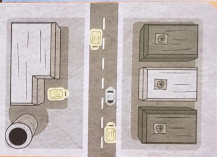
\includegraphics[width=0.5\linewidth]{images/implémentation/road_s_n.png}
        \caption{Route du Nord vers le Sud}
        \label{fig:road_n_s}
    \end{minipage}\hfill
    \begin{minipage}{0.45\textwidth}
        \centering
        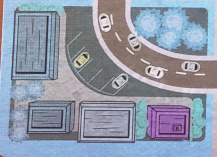
\includegraphics[width=0.5\linewidth]{images/implémentation/road_n_e.png}
        \caption{Route du Nord vers l'Est}
        \label{fig:road_n_e}
    \end{minipage}
\end{figure}

Dans un premier temps les routes on été créées de manière aléatoire, puis de manière fixe pour faciliter les tests ainsi que la liaison des routes sur le graphe des routes.
Le choix de cette implémentation nous permet de facilement savoir vers où pointe la route pour rendre plus accessible l'utilisation de celle-ci.

\subsubsection{Tuile}

Pour l'implémentation des tuiles (appelées \texttt{tile} dans le code) nous avons dû créer deux nouveaux types : \texttt{TileDict<T>} et \texttt{Tile}. Le type \texttt{Tile} est un dictionnaire immutable (MapOf) où les clés sont $roads$ et $neighborhoods$, et leurs attributs sont respectivements \texttt{TileDict<Road>} et \texttt{TileDict<Color>}.
Le type \texttt{TileDict<T>} est lui aussi un dictionnaire immutable, ses clés sont les positions dans la tuile (Nord-Est, Sud-Est, Nord-Ouest, Sud-Ouest) et les attributs sont de type \texttt{T}, où \texttt{T} est : soit de type \texttt{Color} soit de type \texttt{Road}.

La tuile doit posséder un quartier de chaque couleur et une route par quartier sauf sur les quartier vert. Donc lors de la création de la tuile il nous faut d'abord créer le \texttt{TileDict<Color>} pour ensuite placer les routes sur les bonnes couleurs. \\

Exemple : \\

La figure~\ref{fig:tile} est représentée par le dictionnaire : \\
\begin{lstlisting}[language=JavaScript]
{
    roads: {
        nw: {north: false, west: false, south: false, east: false}, 
        ne: {north: true, west: false, south: true, east: false}, 
        se: {north: true, west: true, south: false, east: false}, 
        sw: {north: false, west: true, south: false, east: true}
    },
    neighborhoods: {nw: Green, ne: Grey, se: Red, sw: Blue}
}
\end{lstlisting}

\begin{figure}[h]
    \centering
    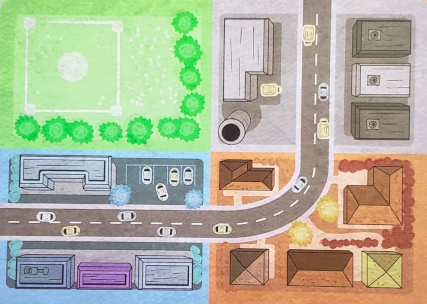
\includegraphics[width=0.3\linewidth]{images/implémentation/exemple_tile.png}
    \caption{Exemple de tuile}
    \label{fig:tile}
\end{figure}

Cette implémention a pour avantage de facilement donner accès aux routes et aux quartiers sans devoir passer par leurs positions dans la tuile puis de récuperer les quartiers puis les routes.

%% Plateau :
\subsection{Représentation du plateau}
\label{subsec:board}

Pour l'implémentation du plateau (appelé \texttt{board} dans le code) nous avons du créer deux nouveaux types : \texttt{Quarter} et \texttt{Board}. Le type \texttt{Quarter} est un dictionnaire immutable où les clés sont \textit{x}, \textit{y}, \textit{road} et \textit{color} et leurs attribus sont respectivements \texttt{number}, \texttt{number} , \texttt{Road} et \texttt{Color}.\\

Nous avons fait ce choix d'implémentation , d'avoir une structure de dictionnaire simple, afin d'avoir un accès rapide et une complexité en O(1) pour la lecture des valeurs.

Le plateau est une liste de "quarter", c'est-à-dire que pour construire la plateau, on décompose une tuile et des coordonnées en quatre "quarter" puis on ajouter chaque "quarter" au plateau.\\

Exemple :

La figure \ref{fig:board_tile} est le plateau constitué d'une seule tuile et représenté par la liste :\\
\begin{lstlisting}[language=JavaScript]
[
    { x: 0, y: 0, road: {
        north: false, west: false, south: false, east: false
    }, color: Green },
    { x: 1, y: 0, road: {
        north: true, west: false, south: true, east: false
    }, color: Grey },
    { x: 0, y: -1, road: {
        north: false, west: true, south: false, east: true
    }, color: Blue },
    { x: 1, y: -1, road: {
        north: true, west: true, south: false, east: false
    }, color: Red }
]
\end{lstlisting}

\begin{figure}[h]
    \centering
    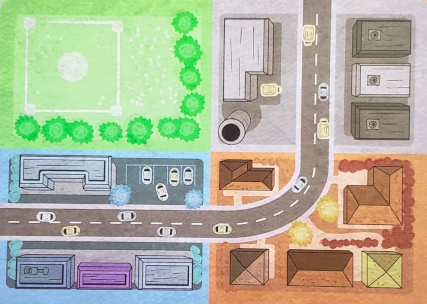
\includegraphics[width=0.3\linewidth]{images/implémentation/exemple_tile.png}
    \caption{Exemple de plateau composé d'une tuile}
    \label{fig:board_tile}
\end{figure}




%% Objectifs
\subsection{Objectifs}
\label{section:objectifs}
Pour jouer à Megalopolis, il faut piocher au hasard, 5 cartes d'objectifs. Chaque carte a un score fixe et des règles qui permettent de gagner ou perdre des points. Pour gagner une partie, il faut avoir plus de points que la somme des scores des cartes d'objectifs. Pour représenter ces cartes, on a une liste des noms de ces objectifs et une liste des scores associés. Ainsi pour calculer le score à atteindre en début de partie, on a juste à additionner les scores des objectifs choisis. 

Pour avoir le choix et se coller au sujet, nous avons implémenté 6 objectifs différents~: 
\begin{itemize}
    \item réduire\_la\_circulation
    \item sortie\_de\_route
    \item arrondissement
    \item passez\_au\_vert
    \item ville fleurie
    \item rocades
\end{itemize}

Nous ne nous sommes pas facilités la tâche, car nous avons également pris des objectifs qui peuvent apporter des points négatifs, ce qui nécessite une bonne stratégie pour pouvoir gagner ! Nous avons donc utilisé les fonctions \texttt{map} et \texttt{reduce} sur les graphes et le plateau pour calculer les points rapportés par ces différents objectifs.

Par soucis de clarté et de pertinence, on ne détaille ici qu'un des objectifs: \texttt{passez\_au\_vert} dont les règles sont les suivantes~:
\begin{itemize}
    \item  $+1$ pt par parc dans la ville
    \item  $-3$ pts par quartier industriel dans la ville
\end{itemize}

Pour calculer le score lié à cette règle , on applique un \texttt{reduce} à la liste des composantes connexes du graphe des couleurs passée en paramètre. La fonction utilisée en paramètre, avec un accumulateur qui vaut 0 initialement, récupère la couleur du premier quartier de chaque composante connexe (puisqu'ils ont par construction, tous la même couleur au sein d'une composante connexe). Si cette couleur est grise (quartier industriel) on enlève $3 \cdot taille\_composante$ à l'accumulateur, alors que si elle est verte, on ajoute $taille\_composante$ à l'accumulateur.
Cette règle "coûte" cher car elle peut apporter beaucoup de points négatifs.

Pour faire le calcul global des points, on doit calculer la somme des points rapportés par toutes les règles. Pour cela, nous avons une fonction appelée \texttt{objectives\_player\_gain}. Elle prend en paramètres~: le graphe des couleurs, le graphe des routes, le plateau de jeu ainsi que la liste des objectifs de la partie. On fait un \texttt{reduce} sur la liste des objectifs, avec un accumulateur à 0 et une fonction qui teste quel est l'objectif testé et en fonction de l'objectif testé, lui applique la fonction qui calcule les points qui correspondent à cet objectif, en lui passant les paramètres nécessaires.

En résumé, implémenter les objectifs a permis l'utilisation de \texttt{reduce} et de \texttt{map} et a été complexifié par la contrainte de pureté.
\subsubsection{Complexité}
Pour les scores, chaque fonction de score recalcule les composantes connexes. Ceci nous impose une complexité plus élevée que si nous ne l'avions fait qu'une seule fois, par manque de temps. Nous avons fait ce choix pour des raisons de facilité, nous voulions dans un premier temps une structure qui fonctionne pour l'améliorer par la suite mais nous nous sommes concentrés sur d'autres points comme le fait d'avoir une stratégie qui fonctionne.

%% Graphes :
\subsection{Graphes}

Pour certains objectifs (voir section~\ref{section:objectifs}), le calcul des points nécessite de lister les composantes connexes, ce qui nous a amené à utiliser des graphes.
Les librairies JavaScript proposées dans le cadre du projet ne fournissant pas d'implémentation de graphes, nous avons dû réaliser notre propre implémentation.

\subsubsection{Représentation des graphes}

Le projet étant à réaliser en TypeScript, nous avons choisi de créer un type de données générique \texttt{Graph<T>}, représentant un graphe non-orienté dont les sommets sont de type~\texttt{T}.

Ce type de données est en réalité un dictionnaire (\texttt{Map}) de la librairie \texttt{Immutable.js}, contenant les champs~:

\begin{itemize}
    \item \texttt{vertices} de type \texttt{List<T>}, qui contient la liste des sommets du graphe,
    \item \texttt{adj} de type \texttt{List<List<T>{>}}, qui est la liste d'adjacence du graphe.
\end{itemize}

% TODO: exemple de représentation d'un graphe ?

Ce type de données est accompagné de quelques fonctions (voir Listing~\ref{listing:interface_graphe}) permettant de construire et lire un graphe~:

\begin{lstlisting}[language=JavaScript, caption = Interface du type \texttt{Graph<T>}, label=listing:interface_graphe]
function initGraph<T>(): Graph<T>;

function addVertex<T>(graph: Graph<T>, vertex: T): Graph<T>;

function addEdge<T>(graph: Graph<T>, indexV1: number, indexV2: number): Graph<T>;

function isEmpty<T>(graph: Graph<T>): boolean

function getVertices<T>(graph: Graph<T>): List<T>

function getVertexNeighbors<T>(graph: Graph<T>, vertexIndex: number): List<T>
\end{lstlisting}


\begin{itemize}
    \item La fonction \texttt{initGraph} créée un \texttt{Graph<T>} vide.
    \item La fonction \texttt{addVertex} ajoute un sommet à un graphe.
    \item La fonction \texttt{addEdge} relie deux sommets entre eux avec une arête. Les deux sommets à relier sont spécifiés par leurs indices dans le tableau \texttt{vertices}.
    \\
    \item La fonction \texttt{isEmpty} revoie \texttt{true} si et seulement si le graphe est vide.
    \item La fonction \texttt{getVertices} renvoie la liste des sommets d'un graphe.
    \item La fonction \texttt{getVertexNeighbors} renvoie la liste des sommets voisins du sommet dont l'indice est passé en paramètre.
\end{itemize}

Ces différentes fonctions permettent de construire et lire un graphe. Les fonctions permettant de supprimer des sommets ou arêtes d'un graphe n'ont pas été implémentées, car elles n'étaient pas nécessaire pour notre usage.

\subsubsection{Composantes connexes}

Certains objectifs nécessitent de déterminer la taille et/ou le nombre de composantes connexes dans un graphe.

Pour cela, nous avons implémenté une fonction récursive \texttt{connexCompRec}, qui effectue plusieurs parcours en profondeur du graphe pour déterminer chaque composante connexe du graphe.

\subsubsection{Cycles}

D'autres objectifs nécessitent de déterminer si une composante est un cycle. Cela se fait en filtrant les composantes et en vérifiant si elles sont cyclique. Pour des raisons de simplification, nous ne vérifions que si elle contient un cycle. En effet, dans le jeu, on n'a que besoin de déterminer les cycles pour des routes, qui ne peuvent pas avoir d'embranchement. Une composante de routes contenant un cycle est alors nécessairement cyclique.

La fonction \texttt{isCycle} détermine s'il existe un cycle dans une composante connexe d'un graphe. Lors d'un parcours en profondeur d'un graphe, on peut détecter la présence d'un cycle si l'on tente de réexplorer un sommet déjà exploré. Cette propriété est utilisée dans notre fonction \texttt{isCycle}.

\subsection{Complexité}
Dans ce projet on détermine la complexité des algorithmes en fonction du nombre d'appels récursifs d'une fonction. On prend par exemple une de nos fonctions centrales au sein de notre projet~: celle de la construction des graphes de couleur ou de route à partir du plateau. L'une des particularités de notre projet est que l'on reconstruit les deux graphes entièrement à chaque fois que l'on ajoute une tuile.

Soit $n$ le nombre de tuile dans le plateau. Pour construire le graphe des couleurs à partir du plateau, on applique un \texttt{reduce} au plateau (sur les quartiers du plateau), avec une fonction qui ajoute les arêtes correspondant au \texttt{Quarter} à l'accumulateur, cet accumulateur est initialement le graphe vide. Ainsi, on a une complexité en $\mathcal{O}(4n)$ car la fonction qui ajoute les arêtes est composé des fonctions \texttt{push} et \texttt{set}, qu'on suppose en temps constant et celle-ci est appelée pour tous les \texttt{Quarter} (4 par tuile).

Une fois cela achevé, on applique un second \texttt{reduce} au plateau, avec la fonction qui retourne le graphe des couleurs si toutes les conditions sont valides. Cette fonction a une complexité en $\mathcal{O}(4n)$. Ainsi la fonction qui génère le graphe couleur est en $\mathcal{O}(8n)$, donc linéaire.

On a fait le choix de reconstruire le graphe entièrement à chaque ajout de tuile pour des raisons de pureté de code et car la complexité de cette fonction reste "raisonnable".

